\documentclass[12pt]{article}

\usepackage[utf8]{inputenc}
\usepackage{newunicodechar}
\usepackage{EngReport}
\usepackage{listings}
\usepackage{cancel}
\usepackage{comment}
\usepackage{amssymb}
\usepackage{amsthm}
\usepackage{amsmath}
\usepackage{graphicx}
\usepackage{setspace}
\usepackage{geometry}
\usepackage{xcolor}  % Required for coloring in listings
\usepackage{tikz}

\graphicspath{{Images/}}
\onehalfspacing
\geometry{letterpaper, portrait, includeheadfoot=true, hmargin=1in, vmargin=1in}

% Define custom colors
\definecolor{myblue}{RGB}{0, 128, 255}
\definecolor{mygreen}{RGB}{34, 139, 34}
\definecolor{myorange}{RGB}{255, 140, 0}
\definecolor{mygray}{RGB}{128, 128, 128}
\definecolor{mypurple}{RGB}{148, 0, 211}
\definecolor{myred}{RGB}{255, 69, 0}

% Configure listings for Python with custom styles
\lstset{
    language=Python,             % Set language to Python
    basicstyle=\ttfamily\small,  % Use a smaller monospace font
    keywordstyle=\color{myblue}\bfseries,  % Keywords in blue and bold
    commentstyle=\color{mygreen}\itshape,  % Comments in green and italic
    stringstyle=\color{myorange},          % Strings in orange
    numberstyle=\color{mygray},            % Line numbers in gray
    identifierstyle=\color{mypurple},      % Functions and variables in purple
    morekeywords={print, len, range},      % Define additional Python keywords
    showstringspaces=false,                % Do not show spaces in strings
    breaklines=true,                       % Enable line breaking
    numbers=left,                          % Add line numbers to the left
    numbersep=5pt,                         % Space between line numbers and code
    frame=single,                          % Add a box around the code
    rulecolor=\color{mygray},              % Frame color
    moredelim=[is][\color{myred}]{@@}{@@}, % Custom inline LaTeX coloring
}

\begin{document}
\renewcommand{\familydefault}{\rmdefault}

\begin{titlepage}
    \null % This is a TeX command that does nothing but is necessary for vfill to work correctly
    \vfill
    \begin{center}
        {\fontsize{35}{48}\selectfont \bfseries CSC263 Tutorial \#8 Exercises}
        \vspace{20pt} \\
        {\LARGE Bipartite Graphs and Algorithms} \\
        \vspace{20pt}
        \textbf{Alexander He Meng}
        \vspace{8pt}
        \\ Prepared for March 14th, 2025
    \end{center}
    \vfill
\end{titlepage}

\pagestyle{fancy}
\fancyhf{}
\setlength{\headheight}{30pt}
\renewcommand{\headrulewidth}{0.4pt}
\renewcommand{\footrulewidth}{0.4pt}
\lhead{\large \textbf{CSC263 UTM} \\ \textbf{Tutorial 2 Exercises}}
\rhead{\large \textbf{Winter 2025} \\ \textbf{Prepared for Jan 2025}}
\rfoot{\textbf{Page \thepage}}
\lfoot{}
\pagebreak
\normalsize

\section*{Question 1}
Consider the following AVL tree. What happens if we insert a node 5 into the tree? Which node is the lowest ancestor to become unbalanced? What type of rotations need to be performed to rebalance the tree? Perform the AVL-INSERT carefully step by step.

\begin{center}
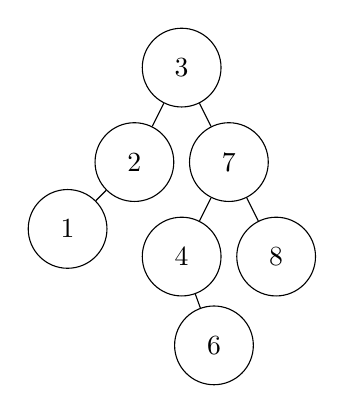
\begin{tikzpicture}[scale=0.8, every node/.style={circle, draw, minimum size=1cm}]
    \node {3}
        child {node {2}
            child [grow=225] {node {1}}
        }
        child {node {7}
            child {node {4}
                child [grow=290]{node {6}}
            }
            child {node {8}}
        };
\end{tikzpicture}
\end{center}

\subsection*{Solution}
When we insert a node 5 into the tree, the tree will look like the following:

\begin{center}
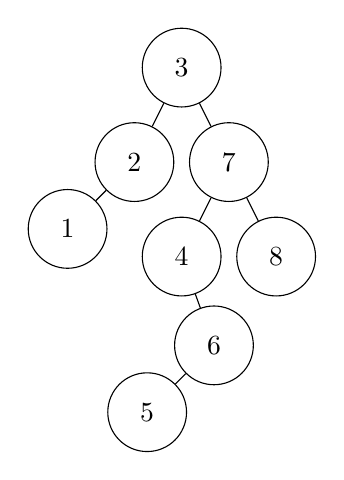
\begin{tikzpicture}[scale=0.8, every node/.style={circle, draw, minimum size=1cm}]
    \node {3}
        child {node {2}
            child [grow=225] {node {1}}
        }
        child {node {7}
            child {node {4}
                child [grow=290]{node {6}} {
                    child [grow=225] {node {5}}
                }
            }
            child {node {8}}
        };
\end{tikzpicture}
\end{center}
\leavevmode\\
The lowest ancestor to become unbalanced is node 4. Since the tree is now right-heavy on node 4 due to the insertion of 5, we need to perform a \textbf{left rotation} at node 4.

\subsubsection*{AVL-Insert Process:}
\begin{enumerate}
    \item Insert 5 as the left child of 6.
    \item Update heights and balance factors.
    \item Detect imbalance at node 4 (balance factor = 2).
    \item Perform a left rotation at node 4, making 6 the new root of the subtree.
\end{enumerate}

After rotations, the final balanced tree is:

\begin{center}
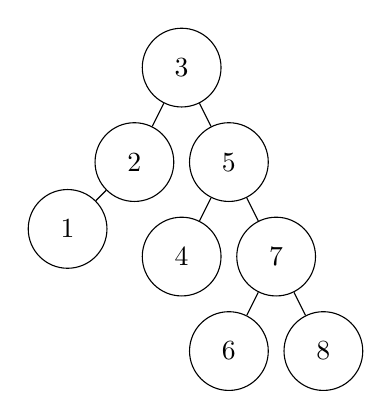
\begin{tikzpicture}[scale=0.8, every node/.style={circle, draw, minimum size=1cm}]
    \node {3}
        child {node {2}
            child [grow=225] {node {1}}
        }
        child {node {5}
            child {node {4}}
            child {node {7}
                child {node {6}}
                child {node {8}}
            }
        };
\end{tikzpicture}
\end{center}

Thus, the tree is balanced again after the left rotation.

\pagebreak

\section*{Question 2}
Consider the following AVL tree. What happens if we delete the node 8 from the tree? What type of rotations are needed to rebalance the tree? What’s the height of the tree before deletion? What’s the height of the tree after deletion?

\begin{center}
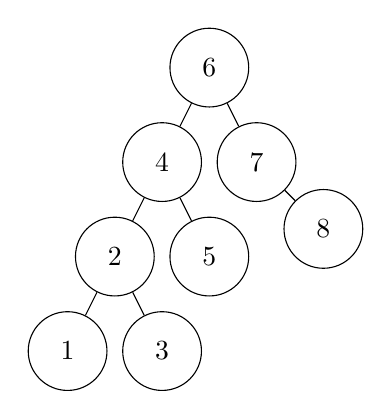
\begin{tikzpicture}[scale=0.8, every node/.style={circle, draw, minimum size=1cm}]
    \node {6}
        child {node {4}
            child {node {2}
                child {node {1}}
                child {node {3}}
            }
            child {node {5}}
        }
        child {node {7}
            child [grow=315] {node {8}}
        };
\end{tikzpicture}
\end{center}

\subsection*{Solution}
When we delete the node 8 from the tree, the tree will look like the following:

\begin{center}
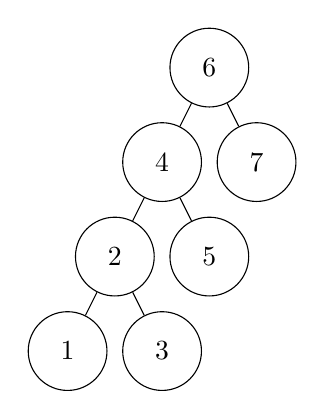
\begin{tikzpicture}[scale=0.8, every node/.style={circle, draw, minimum size=1cm}]
    \node {6}
        child {node {4}
            child {node {2}
                child {node {1}}
                child {node {3}}
            }
            child {node {5}}
        }
        child {node {7}};
\end{tikzpicture}
\end{center}

\subsubsection*{AVL-Deletion Process}
\begin{enumerate}
    \item \textbf{Remove Node 8}
    \begin{itemize}
        \item Since node 8 is a leaf node, we can delete it directly.
    \end{itemize}

    \item \textbf{Update Heights and Balance Factors}
    \begin{itemize}
        \item Before deletion, the height of the right subtree was \textbf{3}.
        \item After deletion, we recalculate the heights:
        \begin{itemize}
            \item The new height of node 7 is \textbf{0} (since it has no children).
            \item The new height of node 4 remains \textbf{3}, and its balance factor is recalculated.
        \end{itemize}
    \end{itemize}

    \item \textbf{Check for Imbalances}
    \begin{itemize}
        \item Node 6 has a balance factor of \textbf{2} (height of left subtree = 4, height of right subtree = 2).
        \item Since the balance factor is \textbf{not} within the range \([-1,1]\), and is left heavy, we need to perform a \textbf{right rotation} at node 4.
    \end{itemize}
\end{enumerate}

After this right rotation, the tree will be balanced again. The final tree will look like the following:
\begin{center}
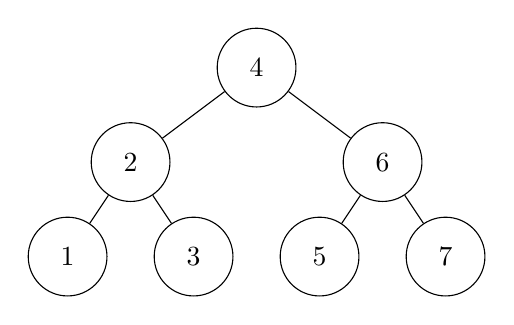
\begin{tikzpicture}[scale=0.8, every node/.style={circle, draw, minimum size=1cm}, sibling distance=4cm]
    \node {4}
        child {node {2} [sibling distance=2cm]
            child {node {1}}
            child {node {3}} 
        }
        child {node {6} [sibling distance=2cm]
            child {node {5}}
            child {node {7}}
        };
\end{tikzpicture}
\end{center}

\begin{enumerate}
    \setcounter{enumi}{3} % Continue numbering from the previous list
    \item \textbf{Perform Right Rotation at Node 6}
    \begin{itemize}
        \item Node 4 becomes the new root.
        \item Node 6 moves down as the right child of 4.
        \item The subtree remains balanced.
    \end{itemize}

    \item \textbf{Final Heights and Balance Factors}
    \begin{itemize}
        \item \textbf{Height before deletion}: \(4\)
        \item \textbf{Height after deletion and rebalancing}: \(3\)
        \item All nodes now have balance factors within \([-1,1]\), ensuring the tree is a valid AVL tree.
    \end{itemize}
\end{enumerate}

Thus, after deleting node 8 and performing a right rotation at node 6, the AVL tree is successfully rebalanced.
\pagebreak

\section*{Question 3}
Consider the following AVL-tree. What happens if we delete the node 2 from the tree? What type of rotations are needed to rebalance the tree? What’s the height of the tree before deletion? What’s the height of the tree after deletion?

\subsection*{Initial AVL Tree}
\begin{center}
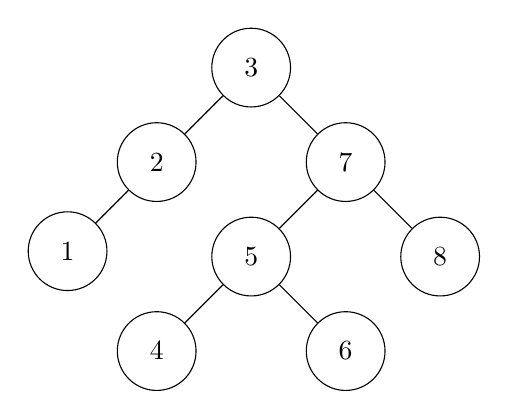
\begin{tikzpicture}[scale=0.8, every node/.style={circle, draw, minimum size=1cm}, sibling distance=3cm]
    \node {3}
        child {node {2}
            child [grow=225, level distance=2cm] {node {1}}
        }
        child {node {7}
            child {node {5}
                child {node {4}}
                child {node {6}}
            }
            child {node {8}}
        };
\end{tikzpicture}
\end{center}

\subsection*{After Deletion of 2 (Replacing with 1)}
\begin{center}
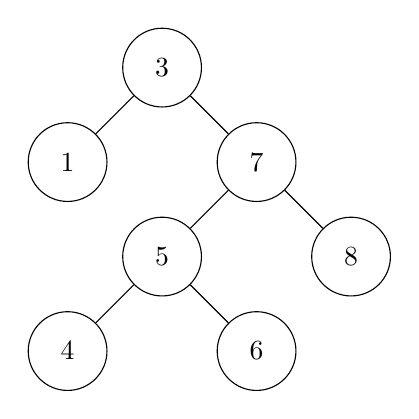
\begin{tikzpicture}[scale=0.8, every node/.style={circle, draw, minimum size=1cm}, sibling distance=3cm]
    \node {3}
        child {node {1}}
        child {node {7}
            child {node {5}
                child {node {4}}
                child {node {6}}
            }
            child {node {8}}
        };
\end{tikzpicture}
\end{center}

\subsection*{After Right Rotation on 5}
\begin{center}
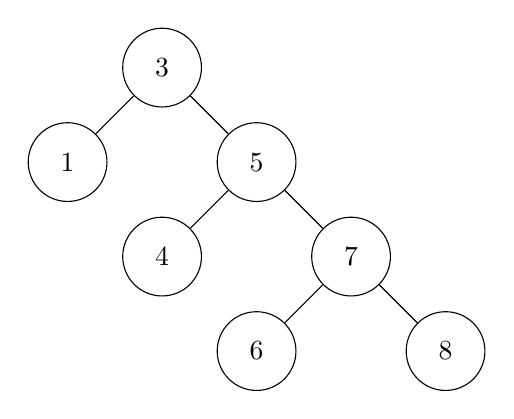
\begin{tikzpicture}[scale=0.8, every node/.style={circle, draw, minimum size=1cm}, sibling distance=3cm]
    \node {3}
        child {node {1}}
        child {node {5}
            child {node {4}}
            child {node {7}} {
                child {node {6}}
                child {node {8}}
            }
        };
\end{tikzpicture}
\end{center}

\subsection*{After Left Rotation on 5 (Final Balanced Tree)}
\begin{center}
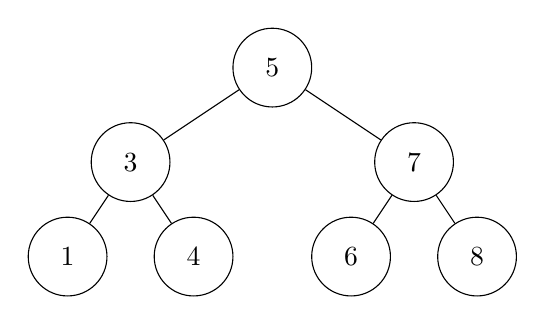
\begin{tikzpicture}[scale=0.8, every node/.style={circle, draw, minimum size=1cm}, sibling distance=3cm]
    \node {5} [sibling distance=4.5cm]
        child {node {3} [sibling distance=2cm]
            child {node {1}}
            child {node {4}}
        }
        child {node {7} [sibling distance=2cm]
            child {node {6}}
            child {node {8}}
        };
\end{tikzpicture}
\end{center}

\subsection*{Height Analysis}
Before deletion, the height of the tree is 4. After deletion and rebalancing, the height becomes 3. The tree is now balanced and satisfies the AVL property.

\pagebreak

\section*{Question 4}
Come up with an example AVL-tree for which deleting a node from the tree causes two levels of double-rotations.

\begin{proof}
\textbf{Solution:} \
\textit{(An AVL-tree example and explanation will be provided here.)}
\end{proof}

\pagebreak

\section*{Question 5}
Draw a picture of the structure of the AVL tree for which deleting a node would cause \( O(\log n) \) rotations, where \( n \) is the number of nodes in the tree.

\begin{proof}
\textbf{Solution:} \
\textit{(Diagram and explanation will be provided here.)}
\end{proof}

\pagebreak

\section*{Question 6}
Suppose in the AVL-INSERT operation, the tree looks like the following right after inserting the new node and before rebalancing.

\begin{center}
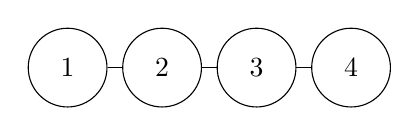
\begin{tikzpicture}[scale=0.8, every node/.style={circle, draw, minimum size=1cm}]
    \node {1}
        child [grow=right] {node {2}
            child [grow=right] {node {3}
                child [grow=right] {node {4}}
            }
        };
\end{tikzpicture}
\end{center}

Since node 2 is the lowest ancestor that is unbalanced, we do a left rotation around 2, which gives us the following tree:

\begin{center}
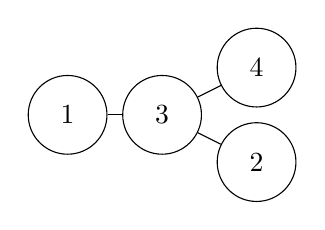
\begin{tikzpicture}[scale=0.8, every node/.style={circle, draw, minimum size=1cm}]
    \node {1}
        child [grow=right] {node {3}
            child {node {2}}
            child {node {4}}
        };
\end{tikzpicture}
\end{center}

This tree is still not AVL, which contradicts what we said in the lecture that AVL-INSERT requires only one level of rotation. What went wrong?

\begin{proof}
\textbf{Solution:} \
\textit{(Explanation of why this contradiction occurs will be provided here.)}
\end{proof}

\end{document}
